\documentclass{article}

\usepackage[utf8x]{inputenc}
\usepackage[english,russian]{babel}
\usepackage{cmap}
\usepackage{commath}
\usepackage{amsmath}
\usepackage{amsfonts}
\usepackage{mathtools}
\usepackage{amssymb}
\usepackage{parskip}
\usepackage{titling}
\usepackage{color}
\usepackage{hyperref}
\usepackage{cancel}
\usepackage{enumerate}
\usepackage{multicol}
\usepackage{graphicx}
\usepackage[font=small,labelfont=bf]{caption}
\usepackage[a4paper, left=2.5cm, right=1.5cm, top=2.5cm, bottom=2.5cm]{geometry}

\graphicspath{ {./images/} }
\setlength{\droptitle}{-3cm}
\hypersetup{ colorlinks=true, linktoc=all, linkcolor=blue }
\pagenumbering{arabic}

\begin{document}
    \section{Производная и дифференциал}
    \subsection{Определение производной. Ее физический и геометрический смысл.}

    \( y = S(t) \) --- закон движения материальной точки. 

    \( v_\textrm{средняя} = \frac{S(t_2) - S(t_1)}{t_2 - t_1} = \begin{cases}
        t_1 = t\\
        t_2 = t + \Delta t
    \end{cases} = \frac{S(t + \Delta t)}{\Delta t} \)

    Для \( y = f(x) \) можем рассмотреть среднюю сокрость изменения скорости.

    \( v_\textrm{средняя} = \frac{f(x + \Delta x) - f(x)}{\Delta x} \)

    В физике мы рассматриваем мгновенную скорость:
    
    \( v_\textrm{мгновенная} = \lim_{\Delta t \to 0} \frac{S(t + \Delta t) - S(t)}{\Delta t} \)
    
    А в математике:
    
    \(\lim_{\Delta x \to 0} \frac{f(x+\Delta x)-f(x)}{\Delta x}\)
    
    \textbf{Определение.} \( \lim_{\Delta x \to 0} \frac{f(x + \Delta x) - f(x)}{\Delta x} \) (если он существует) называется производной функции \( y = f(x) \) в точке \(x\).

    \textbf{Обозначение.} \( \lim_{\Delta x \to 0} \frac{f(x + \Delta x) - f(x)}{\Delta x} = f'(x) \)

    Также существуют другие обозначения производной \( y = f(x) \): \( \dot{y};\ y';\ \frac{df}{dx} \) и т.д.

    Причем \( f(x + \Delta x) - f(x) \) обозначают за \(\Delta y\)
    
    \(\Delta x\) может быть как больше, так и меньше нуля.

    \textbf{Примеры.}

    \begin{enumerate}
        \item \(y = c = const\)

            \(y'(x) = \lim_{\Delta x \to 0}{\frac{y(x+\Delta x)}{\Delta x}} = 0\)
            \\\(\Delta y = c - c = 0\)
        
        \item \( y = cx,\ c = const \)

            \(\Delta y = c(x + \Delta x) - cx = c \Delta x\)

            \(\lim_{\Delta x \to 0}{\frac{\Delta y}{\Delta x}} = \lim_{\Delta x \to 0}{\frac{c \cancel{\Delta x}}{\cancel{\Delta x}}} = c\)

            \((cx)' = c\)
        
        \item \( y = x^n \)
            
            \( \Delta y = (x + \Delta x)^n - x^n = \binom{0}{n} x^n (\Delta x)^0 + \binom{1}{n} x^{n - 1} \Delta x + \binom{2}{n} x^{n - 2} (\Delta x)^2 + \binom{3}{n} x^{n - 3} (\Delta x)^3 + ... + \binom{n}{n} x^0 (\Delta x)^n - x^n = n x^{n - 1} \Delta x + \binom{2}{n} x^{n - 2} (\Delta x)^2 + \binom{3}{n} x^{n - 3} (\Delta x)^3 + ... + \binom{n}{n} x^0 (\Delta x)^n \)

            \( \lim_{\Delta x \to 0} \frac{\Delta y}{\Delta x} = \lim_{\Delta x \to 0} (n x^{n - 1} + \binom{2}{n} x^{n - 2} \Delta x + \binom{3}{n} x^{n - 3} (\Delta x)^2 + ... ) = n x^{n - 1} \)

            \( y' = n x^{n - 1}, n \in \mathbb{N} \)

        \item \(y = \sin x\)
        
            \(\lim_{\Delta x \to 0}{\frac{\sin(x+\Delta x) - \sin x}{\Delta x}} = \lim_{\Delta x \to 0}{\frac{2\sin\frac{x + \Delta x - x}{2}\cos\frac{x + \Delta x + x}{2}}{\Delta x}} = \lim_{\Delta x \to 0}{\frac{\not 2 \sin\frac{\Delta x}{2}\cos(x+\frac{\Delta x}{2})}{\not 2 \frac{\Delta x}{2}}} = \cos x\)
            
            \((\sin x)' = \cos x\)

        \item \( y = tg(x) \)
        
            \( \Delta y = tg(x + \Delta x) - tg(x) = \frac{sin(x + \Delta x)}{cos(x + \Delta x)} - \frac{sin(x)}{cos(x)} = \frac{sin(x + \Delta x)cos(x) - cos(x + \Delta x)sin(x)}{cos(x + \Delta x)cos(x)} = \frac{sin(x + \Delta x - x)}{cos(x + \Delta x)cos(x)} \)

            \( \lim_{\Delta x \to 0} \frac{\Delta y}{\Delta x} = \lim_{\Delta x \to 0} \frac{sin(\Delta x)}{\Delta x cos(x + \Delta x)cos(x)} = \frac{1}{cos(x)^2} \)
        
        \item \((\ctg x)' = \frac{-1}{\sin(x)^2}\)
        \item \(y = ln(x)\)

            \(\lim_{\Delta x \to 0}{\frac{\ln(x+\Delta x) - \ln x}{\Delta x}} =\)

            \(= \lim_{\Delta x \to 0}{\frac{\ln\frac{x + \Delta x}{x}}{\Delta x}} =\)

            \(= \lim_{\Delta x \to 0}{\frac{\ln(1+\frac{\Delta x}{x})}{\Delta x}} =\)

            \(= \lim_{\Delta x \to 0}{\frac{\frac{\cancel{\Delta x}}{x}\ln(1+\frac{\Delta x}{x})^\frac{x}{\Delta x}}{\cancel{\Delta x}}} =\)
            
            \(= \frac{1}{x}\lim_{\Delta x \to 0}{\ln(1 + \frac{\Delta x}{x})^\frac{x}{\Delta x}} = \frac{1}{x}\ln e = \frac{1}{x}\)
        
    \end{enumerate}

    \textbf{Лемма 1.} Если \(y = f(x)\) имеет в некоторой точке \(x\) производную (конечную), то \( y = f(x) \) непрерывна в этой точке.

    \( \uparrow\ \exists\ f'(x) = \lim_{\Delta x \to 0} \frac{f(x + \Delta x) - f(x)}{\Delta x} \) 

    Тогда \( \frac{f(x + \Delta x) - f(x)}{\Delta x} = f'(x) + \alpha(\Delta x)\quad (\alpha \xrightarrow[\Delta x \to 0]{} 0) \)

    \( f(x + \Delta x) - f(x) = f'(x)\Delta x + \alpha(\Delta x)\Delta x \)

    При \( \Delta x \to 0 \)

    \( \lim_{\Delta x \to 0} [f(x + \Delta x) - f(x)] = 0 \)

    \( \lim_{\Delta x \to 0} f(x + \Delta x) = f(x) \), т.е. \( f(x) \) --- непрерывна. \( \downarrow \)

    \textbf{Лемма 2.} Обратное к Л.1 не верно. 
    
    Докажем, что функция \( y = \abs{x} \) не имеет производную в \( x = 0 \)

    \( \lim_{\Delta x \to 0+} \frac{f(0 + \Delta x) - f(0)}{\Delta x} = \lim{\Delta x \to 0+} \frac{\abs{x}}{\Delta x} = \lim_{\Delta x \to 0+} \frac{\Delta x}{\Delta x} = 1 \)

    \( \lim_{\Delta x \to 0-} \frac{f(0 + \Delta x) - f(0)}{\Delta x} = \lim_{\Delta \to 0-} \frac{\abs{\Delta x}}{\Delta x} = \lim_{\Delta x \to 0-} \frac{-\Delta x}{\Delta x} = -1 \)

    \( 1 \neq -1 \Rightarrow \not\exists \lim_{\Delta x \to 0} \frac{\Delta y}{\Delta x} \)

    \subsubsection{Геометрический смысл производной}

    \begin{enumerate}
        \item 
        
            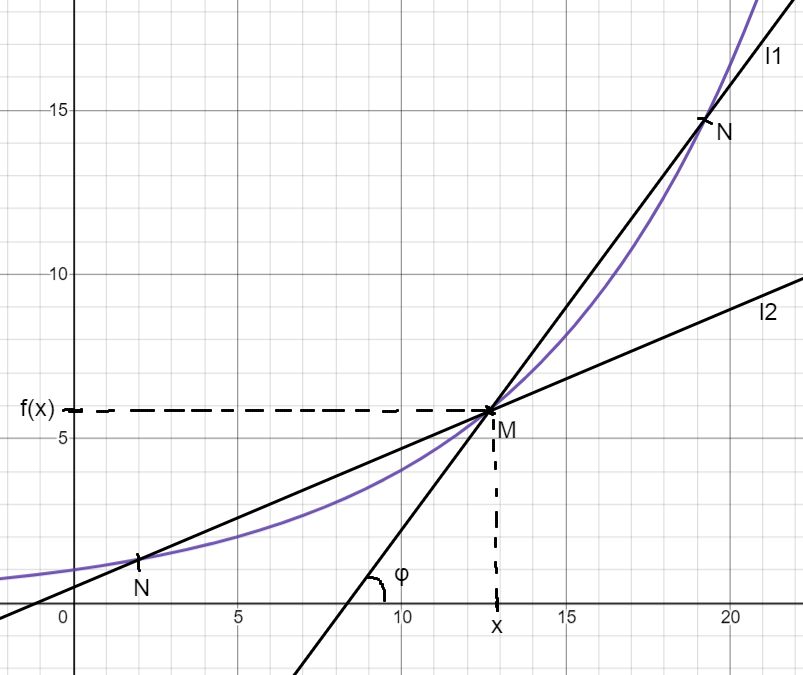
\includegraphics[scale=0.35]{11_1_8_1.png}

            Рассмотрим секущие \( MN \), где \( N \in \textrm{Г}_{f} \)

            Будем \( N \to M \)

            \textbf{Определение.} Предельное положение секущей (если оно существует) \( MN \) при стремлении \( N \) к \( M \) назовем касательной к кривой \( y = f(x) \) в точке \( M \).
            
            \( M \in \) всем секущим для однозначного определения, еще понадобится угол. \( \lim_{N \to M} \phi = \alpha \)

        \item Связь между касательной и производной в точке с абсциссой \( x_0 \). 
        
            \( f'(x) \stackrel{\text{df}}{=} \lim_{\Delta x \to 0} \frac{f(x_0 + \Delta x) - f(x_0)}{\Delta x} = \lim_{\Delta x \to 0; N \to M} tg(\phi) = tg(\alpha) = k\)

            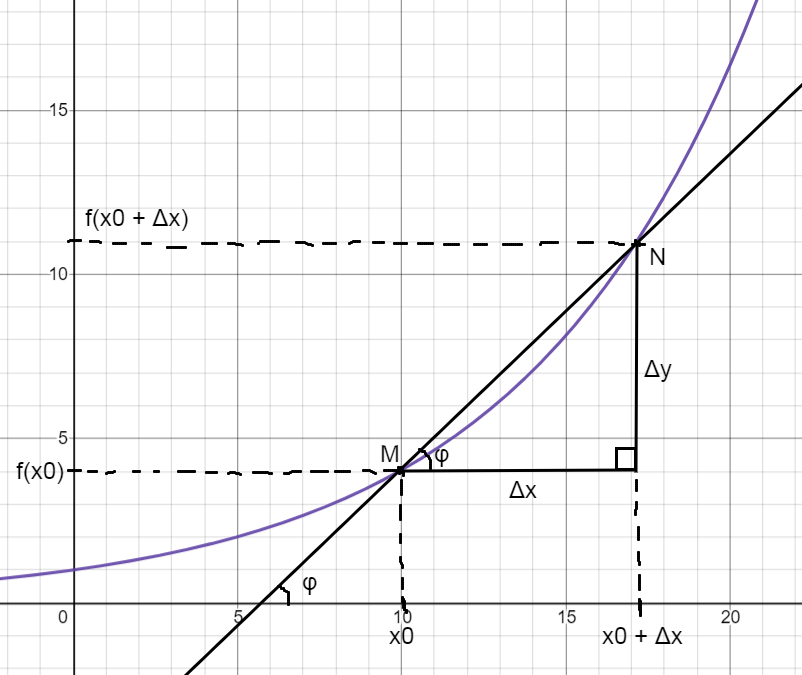
\includegraphics[scale=0.35]{11_1_8_2.png}

            \( tg(\phi) = \frac{\Delta y}{\Delta x} = \frac{f(x_0 + \Delta x) - f(x_0)}{\Delta x} \)

            \( N \to M \Leftrightarrow \Delta x \to 0 \)

            \textbf{Таким образом, производная функции в точке равна тангенсу угла наклона касательной, проведённой в этой точке.}

        \item Уравнение касательной 

            \( tg(\alpha) = f'(x_0) = \frac{y - y_0}{x - x_0} \Rightarrow y = f'(x_0)(x - x_0) + f(x_0) \)
    \end{enumerate}

    \subsection{Правила вычисления производных}

    \textbf{Утверждение.} \( u;\ v \) имеют производные в точке \(x\)

    \begin{enumerate}
        \item \( (u \pm v)' = u' \pm v' \)
        
            \( x \to x + \Delta x \)

            \( u \to u + \Delta u \)

            \( v \to v + \Delta v \)

            \( y = u + v \to u + \Delta u + v + \Delta v \)

            \( \Delta y = (u + \Delta u + v + \Delta v) - (u + v) = \Delta u + \Delta v \)

            \( \lim_{\Delta x \to 0} \frac{\Delta y}{\Delta x} = \lim_{\Delta x \to 0} (\frac{\Delta u + \Delta v}{\Delta x}) = lim_{\Delta x \to 0} (\frac{\Delta u}{\Delta x} + \frac{\Delta v}{\Delta x}) = u' + v' \)

        \item \( (cu)' = cu' \)
        
            \( x \to x + \Delta x \)

            \( u \to u + \Delta u \)

            \( y = cu \to c(u + \Delta u) \)

            \( \Delta y = c(u + \Delta u) - cu = c\Delta u \)

            \( \lim_{\Delta x \to 0} \frac{c\Delta u}{\Delta x} = cu' \)

            \textbf{Пример.}

            \((log_a x)' = (\frac{ln(x)}{ln(a)})' = \frac{1}{ln(a)}(ln(x))' = \frac{1}{x ln(a)} \)

        \item \( (uv)' = u'v + uv' \)
        
            \( x \to x + \Delta x \)

            \( u \to u + \Delta u \)

            \( v \to v + \Delta v \)

            \( \Delta y = (u + \Delta u)(v + \Delta v) - uv = u\Delta v + \Delta uv + \Delta u \Delta v \)

            \(\lim_{\Delta x \to 0}{\frac{u\Delta v + \Delta u v + \Delta u \Delta v}{\Delta x}} = uv' + vu' + u'\lim_{\Delta x \to 0}{\Delta v} = uv' + i'v + 0\)

        \item \( (\frac{u}{v})' = \frac{u'v - uv'}{v^2}  \)
        
            \( x \to x + \Delta x \)
            
            \( u \to u + \Delta u \)

            \( v \to v + \Delta v \)

            \( \Delta y = \frac{u + \Delta u}{v + \Delta v} - \frac{u}{v} = \frac{uv + v\Delta u - uv - u\Delta v}{v(v + \Delta v)} \)
            
            \(\lim_{\Delta x \to 0}{\frac{\Delta y}{\Delta x}} = \lim_{\Delta x \to 0}{\frac{v\Delta u - u\Delta v}{\Delta x}*\frac{1}{v(v+\Delta v)}} = (u'v - uv')\lim_{\Delta x \to 0}{\frac{1}{v(v+\Delta v)}} = \frac{u'v - uv'}{v^2}\downarrow\)
        
            \textbf{Пример.}
            
            \( (tg(x))' = (\frac{sin(x)}{cos(x)})' = \frac{(sin(x))'cos(x) - sin(x)(cos(x))'}{cos(x)^2} = \frac{cos(x)^2 + sin(x)^2}{cos(x)^2} = \frac{1}{sin(x)^2} \)
    \end{enumerate}
    
    \textbf{Утверждение.} Пусть заданы \( y = f(u) \) и \( u = \phi(x) \), имеют производную \(u\) в точке \(x\), \(y\) в \(u = f(x)\) и \( \exists\ F(x) = y = f(\phi(x)) \), тогда \(\exists\) производная \(F_x(x):\ F_x(x) = f_u'(u)\phi_x' = f_u'(\phi(x))\phi_x' \)
    
    \(y = f(u)\) имеет производную; \(\exists \lim_{\Delta u \to 0}{\frac{f(u+\Delta u) - f(u)}{\Delta u}} = \lim_{\Delta u \to 0}{\frac{\Delta y}{\Delta u}} = f_u'\)

    \textbf{Замечание.}
    \( \frac{-\pi}{2} < \phi < \frac{\pi}{2} \)

    \( \phi \to \alpha \)

    \( tg(\phi) \to tg(\alpha) \)

    \( N \to M \)
\end{document}
